%%%% Paramétrage du TD %%%%
\def\xxactivite{ \ifprof {Application 3 -- Corrigé } \else  Application 3\fi} % \normalsize \vspace{-.4cm}
\def\xxauteur{\textsl{Xavier Pessoles}}


%\def\xxnumchapitre{Chapitre 1 \vspace{.2cm}}
%\def\xxchapitre{\hspace{.12cm} Introduction à la dynamique du solide indéformable}

\def\xxcompetences{%
\textsl{%
\textbf{Savoirs et compétences :}\\
\begin{itemize}[label=\ding{112},font=\color{bleuxp}] 
\item Mod2.C18.SF1 : Déterminer l’énergie cinétique d’un solide, ou d’un ensemble de solides, dans son mouvement par rapport à un autre solide.
\item Res1.C1.SF1 : Proposer une démarche permettant la détermination de la loi de mouvement.
\end{itemize}
}}
\def\xxtitreexo{Application 3 --Axe numérique}
\def\xxsourceexo{\hspace{.2cm}}%\footnotesize{Concours Commun Mines Ponts 2016}}

%\def\xxauteur{\textsl{Xavier Pessoles}}

\def\xxfigures{
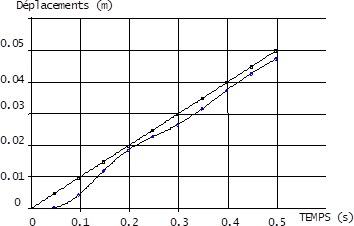
\includegraphics[width=.6\linewidth]{fig_11}
}%figues de la page de garde


\iflivret
\input{\repRel/Style/pagegarde_TD}
\else
\pagestyle{empty}


%%%%%%%% PAGE DE GARDE COURS
\ifcours
\begin{tikzpicture}[remember picture,overlay]
\node at (current page.north west)
{\begin{tikzpicture}[remember picture,overlay]
\node[anchor=north west,inner sep=0pt] at (0,0) {\includegraphics[width=\paperwidth]{\thechapterimage}};
\draw[anchor=west] (-2cm,-8cm) node [line width=2pt,rounded corners=15pt,draw=ocre,fill=white,fill opacity=0.6,inner sep=40pt]{\strut\makebox[22cm]{}};
\draw[anchor=west] (1cm,-8cm) node {\huge\sffamily\bfseries\color{black} %
\begin{minipage}{1cm}
\rotatebox{90}{\LARGE\sffamily\textsc{\color{ocre}\textbf{\xxnumpartie}}}
\end{minipage} \hfill
\begin{minipage}[c]{14cm}
\begin{titrepartie}
\begin{flushright}
\renewcommand{\baselinestretch}{1.1} 
\Large\sffamily\textsc{\textbf{\xxpartie}}
\renewcommand{\baselinestretch}{1} 
\end{flushright}
\end{titrepartie}
\end{minipage} \hfill
\begin{minipage}[c]{3.5cm}
{\large\sffamily\textsc{\textbf{\color{ocre} \discipline}}}
\end{minipage} 
 };
\end{tikzpicture}};
\end{tikzpicture}


\begin{tikzpicture}[overlay]
\node[shape=rectangle, 
      rounded corners = .25 cm,
	  draw= ocre,
	  line width=2pt, 
	  fill = ocre!10,
	  minimum width  = 2.5cm,
	  minimum height = 3cm,] at (18cm,0) {};
\node at (17.7cm,0) {\rotatebox{90}{\textbf{\Large\color{ocre}{\classe}}}};
%{};
\end{tikzpicture}

\vspace{3.5cm}

\begin{tikzpicture}[remember picture,overlay]
\draw[anchor=west] (-2cm,-6cm) node {\huge\sffamily\bfseries\color{black} %
\begin{minipage}{2cm}
\begin{center}
\LARGE\sffamily\textsc{\color{ocre}\textbf{\xxactivite}}
\end{center}
\end{minipage} \hfill
\begin{minipage}[c]{15cm}
\begin{titrechapitre}
\renewcommand{\baselinestretch}{1.1} 
\Large\sffamily\textsc{\textbf{\xxnumchapitre}}

\Large\sffamily\textsc{\textbf{\xxchapitre}}
\vspace{.5cm}

\renewcommand{\baselinestretch}{1} 
\normalsize\normalfont
\xxcompetences
\end{titrechapitre}
\end{minipage}  };
\end{tikzpicture}
\vfill

\begin{flushright}
\begin{minipage}[c]{.3\linewidth}
\begin{center}
\xxfigures
\end{center}
\end{minipage}\hfill
\begin{minipage}[c]{.6\linewidth}
\startcontents
\printcontents{}{1}{}
\end{minipage}
\end{flushright}

\begin{tikzpicture}[remember picture,overlay]
\draw[anchor=west] (4.5cm,-.7cm) node {
\begin{minipage}[c]{.2\linewidth}
\begin{flushright}

\includegraphics[width=2cm]{png/logoCC}
\end{flushright}
\end{minipage}
\begin{minipage}[c]{.2\linewidth}
\textsl{\xxauteur} \\
\textsl{\classe}
\end{minipage}
 };
\end{tikzpicture}
\newpage
\pagestyle{fancy}

\newpage
\pagestyle{fancy}

\else
\fi


%%%%%%%% PAGE DE GARDE TD
\iftd
%\begin{tikzpicture}[remember picture,overlay]
%\node at (current page.north west)
%{\begin{tikzpicture}[remember picture,overlay]
%\draw[anchor=west] (-2cm,-3.25cm) node [line width=2pt,rounded corners=15pt,draw=ocre,fill=white,fill opacity=0.6,inner sep=40pt]{\strut\makebox[22cm]{}};
%\draw[anchor=west] (1cm,-3.25cm) node {\huge\sffamily\bfseries\color{black} %
%\begin{minipage}{1cm}
%\rotatebox{90}{\LARGE\sffamily\textsc{\color{ocre}\textbf{\xxnumpartie}}}
%\end{minipage} \hfill
%\begin{minipage}[c]{13.5cm}
%\begin{titrepartie}
%\begin{flushright}
%\renewcommand{\baselinestretch}{1.1} 
%\Large\sffamily\textsc{\textbf{\xxpartie}}
%\renewcommand{\baselinestretch}{1} 
%\end{flushright}
%\end{titrepartie}
%\end{minipage} \hfill
%\begin{minipage}[c]{3.5cm}
%{\large\sffamily\textsc{\textbf{\color{ocre} \discipline}}}
%\end{minipage} 
% };
%\end{tikzpicture}};
%\end{tikzpicture}

%%%%%%%%%% PAGE DE GARDE TD %%%%%%%%%%%%%%%
%\begin{tikzpicture}[overlay]
%\node[shape=rectangle, 
%      rounded corners = .25 cm,
%	  draw= ocre,
%	  line width=2pt, 
%	  fill = ocre!10,
%	  minimum width  = 2.5cm,
%	  minimum height = 2.5cm,] at (18.5cm,0) {};
%\node at (17.7cm,0) {\rotatebox{90}{\textbf{\Large\color{ocre}{\classe}}}};
%%{};
%\end{tikzpicture}

% PARTIE ET CHAPITRE
%\begin{tikzpicture}[remember picture,overlay]
%\draw[anchor=west] (-1cm,-2.1cm) node {\large\sffamily\bfseries\color{black} %
%\begin{minipage}[c]{15cm}
%\begin{flushleft}
%\xxnumchapitre \\
%\xxchapitre
%\end{flushleft}
%\end{minipage}  };
%\end{tikzpicture}

% Bandeau titre exo
\begin{tikzpicture}[remember picture,overlay]
\draw[anchor=west] (-2cm,-6cm) node {\huge\sffamily\bfseries\color{black} %
\begin{minipage}{5cm}
\begin{center}
\LARGE\sffamily\color{ocre}\textbf{\textsc{\xxactivite}}

\begin{center}
\xxfigures
\end{center}

\end{center}
\end{minipage} \hfill
\begin{minipage}[c]{12cm}
\begin{titrechapitre}
\renewcommand{\baselinestretch}{1.1} 
\large\sffamily\textbf{\textsc{\xxtitreexo}}

\small\sffamily{\textbf{\textit{\color{black!70}\xxsourceexo}}}
\vspace{.5cm}

\renewcommand{\baselinestretch}{1} 
\normalsize\normalfont
\xxcompetences
\end{titrechapitre}
\end{minipage}  };
\end{tikzpicture}

\else
\fi


%%%%%%%% PAGE DE GARDE FICHE
\iffiche
\begin{tikzpicture}[remember picture,overlay]
\node at (current page.north west)
{\begin{tikzpicture}[remember picture,overlay]
\draw[anchor=west] (-2cm,-3.25cm) node [line width=2pt,rounded corners=15pt,draw=ocre,fill=white,fill opacity=0.6,inner sep=40pt]{\strut\makebox[22cm]{}};
\draw[anchor=west] (1cm,-3.25cm) node {\huge\sffamily\bfseries\color{black} %
\begin{minipage}{1cm}
\rotatebox{90}{\LARGE\sffamily\textsc{\color{ocre}\textbf{\xxnumpartie}}}
\end{minipage} \hfill
\begin{minipage}[c]{14cm}
\begin{titrepartie}
\begin{flushright}
\renewcommand{\baselinestretch}{1.1} 
\large\sffamily\textsc{\textbf{\xxpartie} \\} 

\vspace{.2cm}

\normalsize\sffamily\textsc{\textbf{\xxnumchapitre -- \xxchapitre}}
\renewcommand{\baselinestretch}{1} 
\end{flushright}
\end{titrepartie}
\end{minipage} \hfill
\begin{minipage}[c]{3.5cm}
{\large\sffamily\textsc{\textbf{\color{ocre} \discipline}}}
\end{minipage} 
 };
\end{tikzpicture}};
\end{tikzpicture}


\begin{tikzpicture}[overlay]
\node[shape=rectangle, 
      rounded corners = .25 cm,
	  draw= ocre,
	  line width=2pt, 
	  fill = ocre!10,
	  minimum width  = 2.5cm,
%	  minimum height = 2.5cm,] at (18.5cm,0.5cm) {};
	  minimum height = 2.5cm,] at (18.5cm,0cm) {};
\node at (17.7cm,0) {\rotatebox{90}{\textsf{\textbf{\large\color{ocre}{\classe}}}}};
%{};
\end{tikzpicture}



\else
\fi



\fi
\setlength{\columnseprule}{.1pt}

\pagestyle{fancy}
\thispagestyle{plain}

\ifprof
\vspace{5.5cm}
\else
\vspace{5.5cm}
\fi

\def\columnseprulecolor{\color{bleuxp}}
\setlength{\columnseprule}{0.4pt} 
\setcounter{numques}{0}
%%%%%%%%%%%%%%%%%%%%%%%

%\ifprof
%\else
\begin{multicols}{2}
%\fi
%\section*{Exercice 1 -- Lois de Kirchoff}
%\ifprof
%\else
%\fi
%
%\subparagraph*{}
%\textit{Sur le circuit suivant, déterminer les courants dans chacune des branches et la tension aux bornes de tous les dipôles en fonction de $E$ et des différentes résistances $R_i$.}
%\begin{center}
%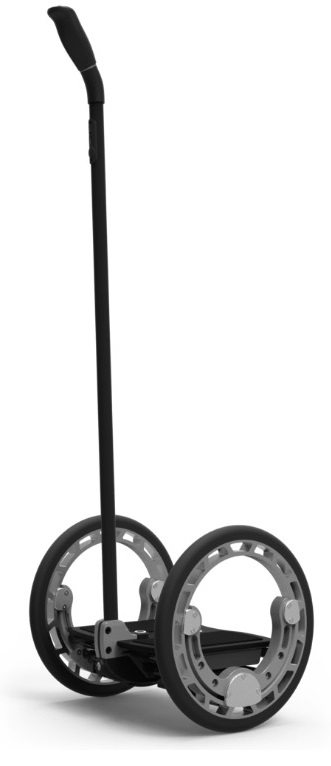
\includegraphics[width=\linewidth]{images/fig_01}
%\end{center}
%
%
%\section*{Exercice 2 -- Résistance équivalente}
%\textit{Déterminer la résistance équivalente du montage suivant.}
%\begin{center}
%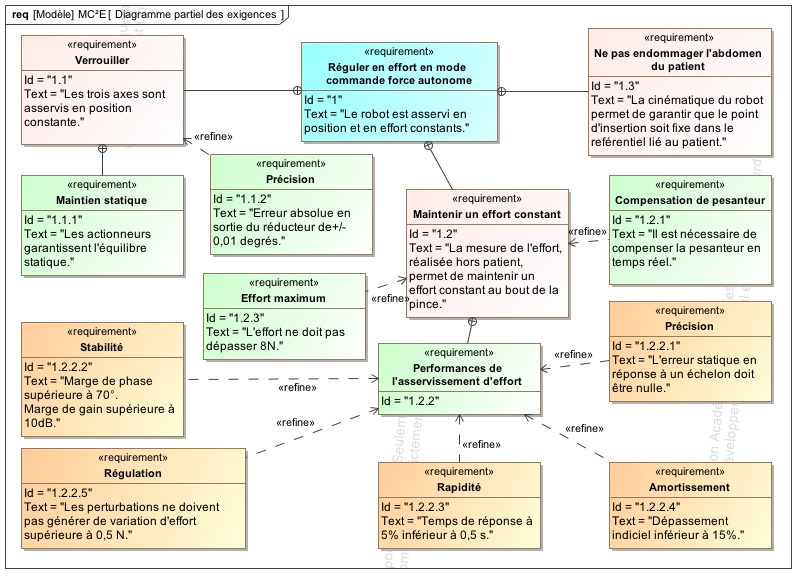
\includegraphics[width=\linewidth]{images/fig_05}
%\end{center}
%




Pour aller rechercher des produits dans leurs rayons, Amazon utilise des axes linéaires afin de déplacer un préhenseur.
\begin{center}
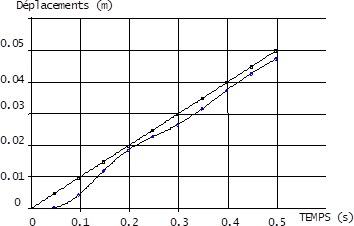
\includegraphics[width=\linewidth]{fig_11}
\end{center}

Les performances dynamique de l'axe demandées sont les suivantes : 
\begin{itemize}
\item vitesse linéaire maximale : $50 \; \text{m}\,\text{min}^{-1}$;
\item accélération linéaire maximale : $9,8 \; \text{m}\, \text{s}^{-2}$.
\end{itemize}

\begin{obj}
L'objectif de ce travail est de déterminer les caractéristiques du moteur (vitesse et couple) permettant d'atteindre ces performances.
\end{obj}

\question{Quelle est la vitesse maximale que l'axe peut atteindre en  $\text{m}\, \text{s}^{-1}$.}
\ifprof
\begin{corrige}
$V = 0,83 \, \text{ms}^{-1}$
\end{corrige}
\else
\fi

\question{Combien de temps l'axe met-il pour atteindre la vitesse maximale ?}
\ifprof
\begin{corrige}
$T_a =0,83/9,8 = 0,08 s$
\end{corrige}
\else
\fi

\question{Quelle distance l'axe parcourt-il pour atteindre la vitesse maximale ?}
\ifprof
\begin{corrige}
\end{corrige}
\else
\fi


\question{Quelle est la longueur minimale à commander pour que l'axe puisse atteindre la vitesse maximale ?}
\ifprof
\begin{corrige}
\end{corrige}
\else
\fi

\question{Proposer une longueur minimale de l'axe pour pouvoir profiter de ses performances dynamiques.}
\ifprof
\begin{corrige}
\end{corrige}
\else
\fi

\question{Tracer le profil de la position, de la vitesse et de l'accélération pour parcourir une distance de 50 cm. On cherchera à atteindre les performances maximales de l'axe. }
\ifprof
\begin{corrige}
\end{corrige}
\else
\fi


Un motoréducteur permet d'entraîner un système poulie -- courroie permettant de déplacer la charge. On considère :
\begin{itemize}
\item une charge de masse $1\; \text{kg}$;
\item un poulie de rayon $5\; \text{cm}$;
\item un réducteur de rapport de transmission $1:20$.
\end{itemize}

\begin{center}
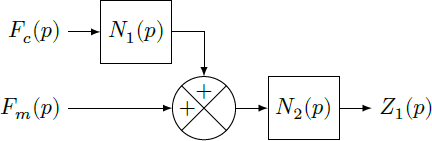
\includegraphics[width=.9\linewidth]{fig_12}
\end{center}

\question{Déterminer le couple à fournir par la poulie pour déplacer la charge lorsque l'accélération est au maximum. }
\ifprof
\begin{corrige}
\end{corrige}
\else
\fi

\question{Déterminer la vitesse et le couple à fournir par le moteur en considérant que l'inertie du motoréducteur est négligeable. }
\ifprof
\begin{corrige}
\end{corrige}
\else
\fi

\question{Donner la méthode permettant de prendre en compte l'inertie $J$ du motoréducteur ? Quel serait l'impact de la prise en compte de cette hypothèse ? }
\ifprof
\begin{corrige}
\end{corrige}
\else
\fi


\end{multicols}